\documentclass[11pt]{article}

\usepackage[margin=1in]{geometry}
\usepackage[T1]{fontenc}
\usepackage{lmodern}
\usepackage{amsmath}
\usepackage{booktabs}
\usepackage{longtable}
\usepackage{tocloft}
\usepackage[hidelinks]{hyperref}
\usepackage{etoolbox}
\usepackage{tikz}

% Start each \section on a new page
% \pretocmd{\section}{\clearpage}{}{}

\setlength{\parindent}{0pt}
\setlength{\parskip}{0.75\baselineskip}

% Dotted leaders in the table of contents
\renewcommand{\cftsecleader}{\cftdotfill{\cftdotsep}}

\title{CO 370 Winter 2026: Group Project Formulation}
\author{
Sa'ad Farooq\thanks{\texttt{s4farooq@uwaterloo.ca}} \and
Maxwell Fang\thanks{\texttt{m34fang@uwaterloo.ca}} \and
Buck Chen\thanks{\texttt{b39chen@uwaterloo.ca}} \and
Timothy Zheng\thanks{\texttt{t54zheng@uwaterloo.ca}}
}

\begin{document}
\maketitle

\section{Topic}
Optimal Power Flow (Direct Current Approximation)

\begin{abstract}
The North American electricity grid operates as a market on a nodal network of energy ``settlement points'' connected by capacity-constrained transmission lines. Participants are generators (gens) and loads, which buy and sell power in real time through an auction process.

The role of the grid operator (RTO) is to ensure economic dispatch of power through a clearing process that tells gens and loads how much power they are allowed (or obligated) to deposit or withdraw from the grid at each settlement point at any given time. Generation and usage capacity is pre-determined 24 hours ahead in the Day-Ahead (DA) market and then additional capacity can be purchased or sold in the Real-time market. 

Since electricity cannot be easily stored, it is instantly delivered across power lines. All market participants are obligated to generate or consume their scheduled amount of electricity to maintain grid stability. Participants must buy or sell in the Real-time market if they are unable to meet their obligations to make their positions whole. Due to the limit in transmission capacity across power lines, power prices tend to be different in different geographical regions, and can be deterministically calculated through LP. 

We propose to write an LP formulation that emulates (approximately) the one run by the grid operator. Our group has access to grid data through a connection from a member's previous co-op. We believe this project is highly relevant given the rapid rise of electricity demand from data centers and manufacturing, and the rise of extreme weather that makes key grid elements more sensitive to catastrophic failures that can result in blackouts.

Optimal power flow has a common approximation assuming DC power flow (the grid is actually run on AC), which allows us to formulate the problem as an LP in the DC model. We hope to implement advanced concepts in OR such as sensitivity analysis, graphs/network flow, and large-scale optimization.

The goal of this project is to simulate an end-to-end market clearing process for a mock electric grid, deriving electricity prices across the grid, and as an extension, clearing one auction round in the electricity derivatives market for a product called Financial Transmission Rights (FTR). We believe this application to be especially enriching to those of us exploring a career in electricity trading, as well as serving as insight into the pricing mechanics of this market in the age of surging power prices due to the rising adoption of datacenters and Artificial Intelligence.
\end{abstract}

\newpage
\tableofcontents
\newpage

\section{Problem Scope, Specification, and Example}



In this project, we focus first on the Day-Ahead (DA) market clearing process. The DA market clearing process involves the grid operator collecting bids from generators (to sell) and loads (to buy) electricity from pre-specified settlement points (pricing nodes) in the power grid for the next 24 hours. In this market, virtual traders also purchase power allocation to be sold later in the real-time market, which settles every 5 minutes in real-time. We decided that this application is out of scope for this assignment and instead we only focus on DA settlement for power and financial derivatives.

It is the role of the RTO to clear this auction, ensuring grid stability while minimizing economic cost. Our goal is to produce the unit allocations (in MW) to each participant and clearing prices (Locational Marginal Prices) of electricity at every node, giving us transparency into the pricing mechanics of this market.

The following is a 3-Node grid example which we will solve manually at the end of the problem specification.

\subsection{3-Node Grid Example}
\begin{center}
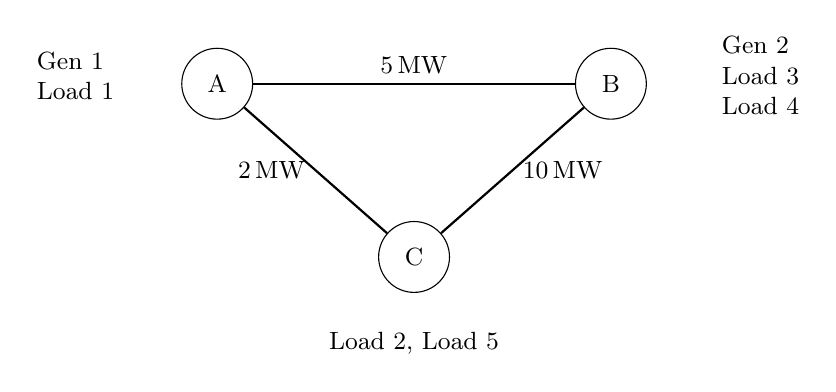
\begin{tikzpicture}[scale=1, every node/.style={font=\small}]
  \node[draw, circle, minimum size=0.9cm] (A) at (0,2.2) {A};
  \node[draw, circle, minimum size=0.9cm] (B) at (5,2.2) {B};
  \node[draw, circle, minimum size=0.9cm] (C) at (2.5,0) {C};

  \draw[thick] (A) -- node[above] {$5\,\mathrm{MW}$} (B);
  \draw[thick] (B) -- node[right] {$10\,\mathrm{MW}$} (C);
  \draw[thick] (A) -- node[left] {$2\,\mathrm{MW}$} (C);

  \node[align=left] at (-1.8,2.3) {Gen 1\\Load 1};
  \node[align=left] at (6.9,2.3) {Gen 2\\Load 3\\Load 4};
  \node[align=left] at (2.5,-1.1) {Load 2, Load 5};
\end{tikzpicture}
\end{center}


Imagine that in our single DA auction, we have the following supply offers.

\begin{center}
\begin{tabular}{lccc}
\toprule
Generator & Node & Offer price (\$/MWh) & Max supply (MW) \\
\midrule
Gen 1 & $A$ & 20 & 12 \\
Gen 2 & $B$ & 45 & 10 \\
\bottomrule
\end{tabular}
\end{center}

and fixed load demand (MUST be filled at economic price):
\begin{center}
\begin{tabular}{lcc}
\toprule
Load & Node & Demand (MW) \\
\midrule
Load 1 & $A$ & 1 \\
Load 2 & $C$ & 5 \\
Load 3 & $B$ & 2 \\
Load 4 & $B$ & 2 \\
Load 5 & $C$ & 6 \\
\bottomrule
\end{tabular}
\end{center}


\section{Data Sources}
Most real-world grid models are confidential, kept behind non-disclosure agreements due to their sensitivity in relation to national security.\footnote{``Electronic copies of the SPP transmission map are currently available to those that provide an Non-Disclosure Agreement (NDA) and appropriate business justification.'', Southwest Power Pool} Therefore for the purpose of this assignment we use the IEEE N-bus systems\footnote{\url{https://github.com/ITI/models/tree/master/electric-grid/physical/reference}} which serve as reference examples to real-world grids as they exist today.

Moreover, as these network models are provided as raw topological specifications, we use \textbf{PowerWorld}, a grid analysis tool to derive shift factors which we use for this project. This calculation is outside the scope of this course, as it does not use LP methods, and is a necessary prerequisite.

We will also be synthesising participant bids and perturbing the grid for exploratory purposes. With this, we have all the necessary inputs to solve our problems.

\section{Constraints}
The power grid is inherently limited by the amount of electricity that can pass through a transmission line. For the purpose of the project, we will only consider constraints as thermal limits to power lines which effectively limit their capacity.

It is the responsibility of the RTO, through the DA clearing process, to ensure the allocations given to the generators and the loads do not overload any transmission line across the grid.

Constraints are defined in \texttt{branches.csv}; see the appendix table preview here: \hyperref[app:branches-preview]{\texttt{branches.csv} preview}.

\section{Contingencies and Monitored Lines}
The RTO also has the additional responsibility to ensure there is no overload across any transmission line in the event an unplanned outage occurs. This is a somewhat common occurrence, as transmission lines can go out for reasons such as wear and tear, extreme weather, trees falling on lines, or circuit breakers being tripped due to line overload. Grid overload can result in temporary power outages, and in severe cases, cascading failure and large-scale blackouts as any significant deviation from the expected generation and load balance can throw off the grid's frequency, damage equipment, and incur high costs to re-sync and restart generators.

Contingencies are always defined with reference to a monitored line. That is, for each contingency and monitored line pair, we open the contingency (so flow across that contingency is 0), and then figure out what the power flow across the rest network will be under the optimized unit allocation. The flow must not exceed the flow limit (constraint) on the monitored line.

The solution employed by RTOs is to evaluate this set of all possible contingencies concurrently, and ensure any cleared auction results in a grid that is stable even if any of the contingencies are activated.

\section{Shift Factor Calculation}
Power Transfer Distribution Factors, a.k.a Shift Factors (sf) are coefficients describing what fraction of electricity will flow through a certain branch (which could comprise multiple lines) if 1 additional MW is injected into the source node and 1 additional MW is withdrawn from the sink node.

In PowerWorld, shift factors are calculated with reference to a fixed slack bus $k$ and are defined per node. 

That is, in the PowerWorld data, shift factors are defined as $\text{sf}_{i \rightarrow k}$. 

Then we can derive for any two nodes $a$, $b$ in the network $\text{sf}_{a \rightarrow b} = \text{sf}_{a \rightarrow k} - \text{sf}_{b \rightarrow k}$


\newpage
\section{Day-Ahead Clearing process}

Ignoring the objective, currently we try to optimize under X, a matrix with the unit allocations for each participant on each node.

The total power flowing on a directed branch (path) with source node $i$ and sink node $j$ is
\[
  \mathrm{flow}_{i\rightarrow j}
  = \sum_{s\in\mathcal{N}} \left(\mathrm{sf}^{(s)}_{i\rightarrow j}\right)\,\mathrm{inj}_s,
\]
where $\mathcal{N}$ is the set of nodes, $\mathrm{sf}^{(s)}_{i\rightarrow j}$ denotes the shift factor on branch $i\to j$ with reference node $s$, and $\mathrm{inj}_s$ is the net injection at node $s$.

Note that negative flow just means the power goes in the opposite direction. That is, the flow from $b$ to $a$ is the same as the negative of the flow from $a$ to $b$. However to save on computation we just need to check if the absolute value is within the node constraint, meaning we need to double each constraint when we implement.

Next, we need to formulate the contingencies. Like the calculation above, we have a matrix of shift factors, but this time each column is a monitored line given some contingency being open in the constraint definition list, while the previous matrix had columns equal to each branch.

\section{Shadow Price Calculation}

\begin{itemize}
  \item Let $\lambda$ denote the dual variable associated with the (system-wide) power-balance constraint.
  \item Let $\mu_l$ denote the dual variable (shadow price) associated with the transmission constraint for line $l$ (binding only when the line is congested).
\end{itemize}
After solving the LP, we will record $\lambda$ and the vector $\{\mu_l\}_{l\in\text{Lines}}$ and use them in
\[
  \mathrm{LMP}_i = \lambda + \sum_{l\in\text{Lines}} \left(\mathrm{PTDF}_{l,i}\,\mu_l\right).
\]

\newpage
\section{Locational Marginal Price Calculation}

For our project, the locational marginal price (LMP) at bus $i$ is the DC approximation:
\[
  \mathrm{LMP}_i = \lambda + \sum_{l\in\text{Lines}} \left(\mathrm{PTDF}_{l,i}\,\mu_l\right).
\]

\noindent
Where:
\begin{itemize}
  \item $\lambda$ is the dual variable of the system power-balance constraint.
  \item $\mu_l$ is the dual variable (shadow price) of the transmission line constraint for line $l$.
  \item $\mathrm{PTDF}_{l,i}$ is the power transfer distribution factor (shift factor) for line $l$ and bus $i$.
\end{itemize}

\section{FTR Contracts}
Financial Transmission Rights (FTR) are derivative contracts\footnote{\url{https://en.wikipedia.org/wiki/Derivative_(finance)}} where the underlying is the congestion between any two nodes $(a, b)$ in a power grid. Their payout is calculated as

$$\text{Payout} = (LMP_{Sink} - LMP_{Source}) \times \text{Quantity (MW)}$$

where the $(LMP_{Sink} - LMP_{Source})$ is known as congestion.

Congestion is only non-zero in the case where constraints in the DA clearance are binding (the inequality replaced with equality).

The trading of these contracts does not affect the underlying power market, however it is a common tool used by market participants to hedge their operations against congestion costs. If the difference is positive, the contract holder is paid by the RTO. If the difference is negative, the contract holder is obligated to pay the RTO the difference. For example, a utility provider may purchase FTRs to guarantee their customers a fixed price for electricity, which is preferred to power prices that fluctuate daily and are unpredictable. Power plants may also purchase these contracts to guarantee a sale price to lock in their profit margins.

\newpage
\section{FTR Clearance}
The clearing process is formally defined in the references in the Iowa State paper (Ma, et al.) As a summary, the FTR clearing process is mostly similar to the DA clearing process however the unit allocation is not bounded by the generation/demand capacity, but instead the amount of bids and offers, ultimately capped by the transmission capacity of a branch. For example, on a line going from node $A \rightarrow B$ with capacity $100\text{MW}$, up to $150\text{MW}$ of capacity can be cleared for that line, given that for the $50\text{MW}$ of excess capacity sold, there are at least $50\text{MW}$ cleared for $B \rightarrow A$.

\textbf{Rationale} (to why net FTR volume over a line is capped by the transmission limit of the line): Note that the shadow price of a line is going to be 0 if it is not binding (the amount of electricity being transmitted is less than the limit). The shadow price is only going to be non-zero if the line is binding, and the capacity is reached.

Since the RTO only needs to pay out (or receive payment) from the derivative in the case where the congestion is non-zero, and congestion on a line is a linear function of the shadow price on the line (\textbf{TODO:} proof needed), the RTO only wants to sell up to the capacity of the line to ensure they can collect the necessary congestion rent from the difference from the DA market.

\textbf{Why is congestion rent positive? } Generators sometimes sell at a lower price at their pricing node, but electricity purchased at another node (suppose this node has no generation) will be more expensive due to demand at a supply-constrained node; then the buyers pay a higher LMP while the seller only receives the cheaper node's LMP. The "profit" generated by the RTO goes straight into paying FTRs.

\section{Full worked example (end-to-end)}
In this example, it is relatively easy to come up with an optimal solution by inspection.

Note the clearing process flows in the following manner:

\begin{center}
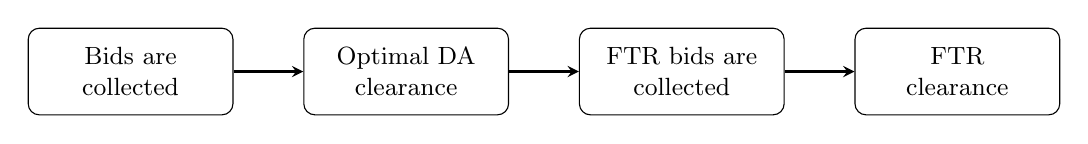
\begin{tikzpicture}[>=stealth, font=\small]
  \node[draw, rounded corners, minimum width=2.6cm, minimum height=1.1cm, align=center] (s1) at (0,0) {Bids are\\collected};
  \node[draw, rounded corners, minimum width=2.6cm, minimum height=1.1cm, align=center] (s2) at (3.5,0) {Optimal DA\\clearance};
  \node[draw, rounded corners, minimum width=2.6cm, minimum height=1.1cm, align=center] (s3) at (7.0,0) {FTR bids are\\collected};
  \node[draw, rounded corners, minimum width=2.6cm, minimum height=1.1cm, align=center] (s4) at (10.5,0) {FTR\\clearance};

  \draw[->, thick] (s1.east) -- (s2.west);
  \draw[->, thick] (s2.east) -- (s3.west);
  \draw[->, thick] (s3.east) -- (s4.west);
\end{tikzpicture}
\end{center}

The DA clearing process works as follows:

\begin{itemize}
    \item \textbf{}
\end{itemize}


\textbf{Potential extensions:} Add already cleared capacity from previous action rounds, bidding on node pairs that are non-adjacent.

\section{DA Clearance LP Formulation}

\subsection{Given}

We consider a power network operated under a DC power flow approximation.
Generation must be dispatched to meet demand at minimum cost while satisfying:

\begin{itemize}
    \item System-wide power balance,
    \item Generator operating limits,
    \item Transmission thermal limits,
    \item $N$-$1$ security constraints (contingency feasibility).
\end{itemize}

The dispatch must remain feasible under all specified contingencies without post-contingency redispatch.

\subsection{Parameters}

\begin{itemize}
    \item $\mathcal{N}$ : Set of buses (nodes)
    \item $\mathcal{L}$ : Set of transmission lines
    \item $\mathcal{G}$ : Set of generators
    \item $\mathcal{D}$ : Set of loads
    \item $\mathcal{K} \subseteq \mathcal{L}$ : Set of contingencies
    \item $c_g$ : Marginal cost of generator $g$
    \item $g_g^{\min}, g_g^{\max}$ : Generation limits
    \item $d_d^{\text{nom}}$ : Nominal demand
    \item $F_l^{\max}$ : Thermal flow limit of line $l$
    \item $PTDF_{l,s}$ : Shift factor of line $l$ with respect to node $s$
    \item $PTDF_{l,s}^{(k)}$ : Shift factor under contingency $k$
    \item $n(g)$ : Node of generator $g$
    \item $n(d)$ : Node of load $d$
\end{itemize}

\subsection{LP Variables}

\begin{itemize}
    \item $g_g \ge 0$ : Power produced by generator $g$
    \item $d_d \ge 0$ : Power served to load $d$
\end{itemize}

 
These variables determine the economic dispatch. Generation variables determine supply, and demand variables allow the model to enforce power balance and load limits.

\section*{LP Objective Function}

\begin{equation}
\min_{g,d} \quad \sum_{g \in \mathcal{G}} c_g g_g
\end{equation}

 
The objective minimizes total generation cost, ensuring the most economical dispatch that satisfies reliability constraints.

\subsection{LP Constraints}

\subsection{System Power Balance}

\begin{equation}
\sum_{g \in \mathcal{G}} g_g
-
\sum_{d \in \mathcal{D}} d_d
= 0
\end{equation}

 
Ensures total generation equals total demand, maintaining physical feasibility of the power system.

\subsection{Generator Capacity Limits}

\begin{equation}
g_g^{\min} \le g_g \le g_g^{\max}
\quad \forall g \in \mathcal{G}
\end{equation}

 
Generators cannot produce below minimum stable output or exceed technical capacity limits.

\subsection{Load Limits}

\begin{equation}
0 \le d_d \le d_d^{\text{nom}}
\quad \forall d \in \mathcal{D}
\end{equation}

 
Prevents serving more than the available demand and ensures non-negativity of consumption.

\subsection{Net Injection Definition}

For each node $s \in \mathcal{N}$:

\begin{equation}
inj_s =
\sum_{g: n(g)=s} g_g
-
\sum_{d: n(d)=s} d_d
\end{equation}

 
Defines nodal net injection used to compute transmission flows via PTDFs.

\subsection{Base-Case Transmission Constraints}

\begin{equation}
- F_l^{\max}
\le
\sum_{s \in \mathcal{N}} PTDF_{l,s} \, inj_s
\le
F_l^{\max}
\quad \forall l \in \mathcal{L}
\end{equation}

 
Ensures no transmission line exceeds its thermal rating under normal operating conditions.

\subsection{Contingency Constraints (N-1 Security)}

\begin{equation}
- F_l^{\max}
\le
\sum_{s \in \mathcal{N}} PTDF_{l,s}^{(k)} \, inj_s
\le
F_l^{\max}
\quad \forall l \in \mathcal{L}, \forall k \in \mathcal{K}
\end{equation}

 
Guarantees that the chosen dispatch remains feasible if any single contingency occurs.  
The same generation dispatch must satisfy all contingency flow limits (no corrective redispatch).

\subsection{Full SCED Formulation}

\begin{align}
\min_{g,d} \quad
& \sum_{g \in \mathcal{G}} c_g g_g
\\[6pt]
\text{s.t.} \quad
& \sum_{g \in \mathcal{G}} g_g
-
\sum_{d \in \mathcal{D}} d_d
= 0
\\[6pt]
& g_g^{\min} \le g_g \le g_g^{\max}
\quad \forall g \in \mathcal{G}
\\[6pt]
& 0 \le d_d \le d_d^{\text{nom}}
\quad \forall d \in \mathcal{D}
\\[6pt]
& -F_l^{\max}
\le
\sum_{s \in \mathcal{N}} PTDF_{l,s}
\left(
\sum_{g: n(g)=s} g_g
-
\sum_{d: n(d)=s} d_d
\right)
\le
F_l^{\max}
\quad \forall l \in \mathcal{L}
\\[6pt]
& -F_l^{\max}
\le
\sum_{s \in \mathcal{N}} PTDF_{l,s}^{(k)}
\left(
\sum_{g: n(g)=s} g_g
-
\sum_{d: n(d)=s} d_d
\right)
\le
F_l^{\max}
\quad \forall l \in \mathcal{L}, \forall k \in \mathcal{K}
\end{align}

\section{FTR Clearance LP}
\subsection{Given}
We consider an FTR auction/clearing problem under a DC power-flow approximation.
The market operator clears a set of FTR bids subject to \textbf{Simultaneous Feasibility Test (SFT)}
constraints so that the awarded FTR portfolio is feasible with respect to transmission thermal limits
in the base case and (optionally) under $N\!-\!1$ contingencies. The clearing maximizes total bid value
(revenue/surplus) subject to network feasibility.

\subsection {Parameters}
\begin{itemize}
  \item $\mathcal{N}$ : Set of buses (nodes)
  \item $\mathcal{L}$ : Set of monitored transmission lines
  \item $\mathcal{K}$ : Set of contingencies (optional). If base-case only, let $\mathcal{K}=\{\text{base}\}$.
  \item $\mathcal{R}$ : Set of FTR bids (each bid is a directed point-to-point right)
  \item $o(r)$ : Source node of bid $r\in\mathcal{R}$
  \item $t(r)$ : Sink node of bid $r\in\mathcal{R}$
  \item $\bar q_r \ge 0$ : Maximum MW quantity that can be awarded for bid $r$
  \item $p_r$ : Bid price (\$/MW) for bid $r$ (willingness-to-pay per MW of FTR)
  \item $F_l^{\max}$ : Thermal flow limit (MW) of line $l\in\mathcal{L}$
  \item $PTDF^{(k)}_{l,s}$ : Shift factor of line $l$ w.r.t. node $s$ under contingency $k\in\mathcal{K}$

\end{itemize}

\subsection*{Variables}
\begin{itemize}
  \item $x_r \ge 0$ : Awarded MW quantity of FTR bid $r\in\mathcal{R}$
\end{itemize}

\subsection*{Objective Function}
\begin{equation}
\max_{x}\ \sum_{r\in\mathcal{R}} p_r\,x_r
\tag{1}
\end{equation}
The objective maximizes total cleared bid value (auction surplus/revenue) subject to SFT feasibility.

\subsection*{Constraints}

\subsubsection*{1. Bid Quantity Limits}
\begin{equation}
0 \le x_r \le \bar q_r \quad \forall r\in\mathcal{R}
\tag{2}
\end{equation}
Awards cannot exceed the bid quantity.

\subsubsection*{2. SFT Line Flow Constraints (Base Case and Contingencies)}
Each awarded FTR $r: o(r)\to t(r)$ is modeled as a \emph{virtual transaction} that injects at $o(r)$ and
withdraws at $t(r)$. Under DC approximation, its contribution to line $l$ (in contingency $k$) is the PTDF
difference:
\[
\Delta PTDF^{(k)}_{l,r} \;=\; PTDF^{(k)}_{l,t(r)} - PTDF^{(k)}_{l,o(r)}.
\]
The simultaneous feasibility test enforces that the \emph{net} effect of all awarded FTRs respects thermal limits:
\begin{equation}
- F_l^{\max}
\le
\sum_{r\in\mathcal{R}} \Big( PTDF^{(k)}_{l,t(r)} - PTDF^{(k)}_{l,o(r)} \Big)\,x_r
\le
F_l^{\max}
\quad \forall l\in\mathcal{L},\ \forall k\in\mathcal{K}.
\tag{3}
\end{equation}

\subsection*{Full FTR Clearance Formulation}
\begin{align}
\max_{x}\quad & \sum_{r\in\mathcal{R}} p_r\,x_r
\tag{4}\\[4pt]
\text{s.t.}\quad
& 0 \le x_r \le \bar q_r \quad \forall r\in\mathcal{R}
\tag{5}\\[4pt]
& - F_l^{\max}
\le
\sum_{r\in\mathcal{R}} \Big( PTDF^{(k)}_{l,t(r)} - PTDF^{(k)}_{l,o(r)} \Big)\,x_r
\le
F_l^{\max}
\quad \forall l\in\mathcal{L},\ \forall k\in\mathcal{K}.
\tag{6}
\end{align}
\newpage

\section{Results}
\textbf{TODO:} Implement in Python, using data in appendix. Collect and Interpret Results

\section{IP Formulation for DA / FTR (first extension)}
\textbf{TODO:} Both DA and FTR markets require users to bid on a curve, giving (pi, qi) price, quantity pairs. We find an optimal solution such that the result is an integer multiple of $0.1\text{MW}$ (the base unit).

\section{Other Extensions}
\begin{enumerate}
    \item MIP for unit allocation given that gens have startup cost, cost-curves
    \item Sensitivity analysis (possible worst states of the grid -> we want to guarantee grid stability.) Which lines can cause the greatest price impact if they suddenly go out for an unexplained reason?
\end{enumerate}

\appendix
\newpage
\section{Appendix: Data Previews}

\subsection{\texttt{branches.csv} preview}\label{app:branches-preview}
\textbf{Summary:} Branch definitions and parameters. Only Limit A applies for now.

\scriptsize
\begin{longtable}{@{}rrrrllcrrrr@{}}
\toprule
ID & From \# & To \# & Ckt & Status & Type & Xfrmr & $R$ & $X$ & $B$ & Limit A \\
\midrule
\endhead
1  & 1 & 2  & 1 & Closed & Line        & NO  & 0.00070 & 0.00123 & 0.00065 & 175.0 \\
2  & 1 & 5  & 1 & Closed & Line        & NO  & 0.02243 & 0.08490 & 0.02440 & 175.0 \\
3  & 2 & 4  & 1 & Closed & Line        & NO  & 0.03361 & 0.12730 & 0.03660 & 175.0 \\
4  & 2 & 6  & 1 & Closed & Line        & NO  & 0.05064 & 0.19201 & 0.05570 & 175.0 \\
5  & 3 & 1  & 1 & Closed & Line        & NO  & 0.05419 & 0.21114 & 0.06130 & 175.0 \\
6  & 3 & 9  & 1 & Closed & Line        & NO  & 0.03148 & 0.11921 & 0.03430 & 175.0 \\
7  & 4 & 9  & 1 & Closed & Line        & NO  & 0.02692 & 0.10779 & 0.02790 & 175.0 \\
8  & 5 & 10 & 1 & Closed & Transformer & YES & 0.02334 & 0.08837 & 0.02540 & 175.0 \\
9  & 7 & 8  & 1 & Closed & Line        & NO  & 0.01614 & 0.06103 & 0.01790 & 175.0 \\
10 & 8 & 9  & 1 & Closed & Line        & NO  & 0.04234 & 0.16482 & 0.04780 & 175.0 \\
\bottomrule
\end{longtable}
\normalsize

\subsection{\texttt{buses.csv} preview}
\textbf{Summary:} Bus-level voltage, angle, generation, and load data.

\scriptsize
\begin{longtable}{@{}rrrrrr@{}}
\toprule
Bus \# & Nom kV & PU Volt & Angle (deg) & Gen (\text{MW}) & Load (\text{MW}) \\
\midrule
\endhead
1  & 138.00 & 1.00000 & 0.00  & 35.85 & 0.00 \\
2  & 138.00 & 0.99783 & 0.01  & 67.00 & 97.00 \\
3  & 138.00 & 0.86395 & 10.75 & 0.00  & 90.00 \\
4  & 138.00 & 0.88721 & -0.42 & 0.00  & 74.00 \\
5  & 138.00 & 0.92693 & -0.22 & 0.00  & 71.00 \\
6  & 138.00 & 0.90837 & 0.39  & 0.00  & 68.00 \\
7  & 138.00 & 0.79668 & -0.58 & 64.00 & 62.00 \\
8  & 230.00 & 0.80581 & -0.87 & 0.00  & 85.00 \\
9  & 138.00 & 0.83528 & 4.98  & 0.00  & 175.00 \\
10 & 138.00 & 0.88216 & 3.72  & 0.00  & 100.00 \\
\bottomrule
\end{longtable}
\normalsize

\subsection{\texttt{ptdf.csv} preview}
\textbf{Summary:} PTDF/shift-factor matrix (rows: buses; columns: branches). Below is a small subset of columns.

\scriptsize
\begin{longtable}{@{}rrrrrr@{}}
\toprule
Bus \# & ETLR & WTLR & 1\,to\,2 & 3\,to\,1 & 1\,to\,5 \\
\midrule
\endhead
1  & 0.0000  & 0.0000  & 0.0000  & 0.0000  & 0.0000 \\
2  & -0.9962 & -1.4054 & -0.9946 & 0.0021  & -0.0033 \\
3  & 1.1629  & 1.0685  & -0.3619 & 0.4416  & -0.1965 \\
4  & -1.7811 & -1.6472 & -0.7309 & 0.1304  & -0.1387 \\
5  & -1.3303 & -1.0981 & -0.2290 & 0.0790  & -0.6920 \\
6  & -1.7217 & -1.9384 & -0.5453 & 0.1377  & -0.3170 \\
7  & -0.6366 & -0.9519 & -0.4875 & 0.2002  & -0.3124 \\
8  & -1.6366 & -1.0722 & -0.4875 & 0.2002  & -0.3124 \\
9  & -0.5991 & -0.5184 & -0.5076 & 0.2391  & -0.2533 \\
10 & -0.6740 & -0.7555 & -0.4673 & 0.1612  & -0.3714 \\
\bottomrule
\end{longtable}
\normalsize

\newpage
\section{References}
\begin{sloppypar}
\noindent
Sun, Junjie, and Leigh Tesfatsion. ``DC Optimal Power Flow Formulation and Solution Using QuadProgJ.'' \textit{ISU Economics Working Paper No. 06014}, revised 1 Mar.\ 2010, Iowa State University. \url{https://faculty.sites.iastate.edu/tesfatsi/archive/tesfatsi/DC-OPF.JSLT.pdf}. Accessed 5 Feb.\ 2026.
\end{sloppypar}

\noindent
ITI. ``models/electric-grid/physical/reference at master \textperiodcentered{} ITI/models.'' \textit{GitHub}. \url{https://github.com/ITI/models/tree/master/electric-grid/physical/reference}. Accessed 5 Feb.\ 2026.

\noindent
Southwest Power Pool. ``SPP Maps Frequently Asked Questions.'' \textit{SPP}. \url{https://www.spp.org/engineering/modeling/spp-maps-frequently-asked-questions/}. Accessed 5 Feb.\ 2026.

\noindent
Ma, Xingwang, David I. Sun, and Andy Ott. ``Implementation of the PJM Financial Transmission Rights Auction Market System.'' \textit{IEEE Power Engineering Society Summer Meeting}, 2002. \url{https://home.engineering.iastate.edu/~jdm/OldInfo/ArevaPJM2002.pdf}. Accessed 5 Feb.\ 2026.

\end{document}
